\chapter{Survey of Anchor Node Placements}

\section{Measuring Location Error}
Before searching for the best anchor node placement we must first define what \emph{best} means, in terms of location error.  First of all, location error is measured as a factor of radio radius (or range).  Since this study addresses range-free networks, and thus relies solely on network connectivity, the actual units of distance do not matter for general study.  What is important to the protocol is how many other nodes in the network fall within the radio radius of a given node.  The average numbers of nodes within range of a each node is known as connectivity.

Every network has its own application requirements, and thus there are many options for what statistics to examine for accessing the quality of locations.  The simplest criteria is to look at the mean location error across all nodes in the network.  For the most part, this is the basis for the results in this study.  However, this assumes that all nodes in the network must be used in the final results.  If the network designers know which nodes have poor locations, they may wish to exclude these nodes from the final results.  Therefore, if the economics of the network deployment allow, it may be beneficial to look at the best, for example, 80\% of nodes in the network.  In practice, the designers do not know which nodes to exclude, so this study also attempts to identify the worst areas of a network for location accuracy, depending on the anchor node placement.  

\section{Coordinate Transformation}
To understand the various hypotheses for the best anchor placement, a basic understanding of how the transformation from local to global coordinate systems must be explained.  After the local networks have been calculated and patched together into a single cohesive network, the anchor nodes are then used. Using Procrustes~\cite{procrustes-matlab} analysis, a linear transformation of translation, reflection, orthogonal rotation, and scaling is determined for the anchor nodes from the calculated to known coordinates. The transformation is then applied to all nodes in the network. Therefore, how well the anchor nodes represent the overall calculated network variability, the better the final locations will be.

\section{Methodology}
For the purposes of testing each hypothesis, randomly generated networks of varying sizes are used.  Unless otherwise specified, all nodes are randomly placed within a square area with an overall density of one node per unit area.  For example, a ten by ten square area will have 100 randomly placed nodes.  Anchor sets are chosen by identifying all possible sets via \emph{n choose k}, where \emph{n} is the number of nodes in the network and \emph{k} is the number of nodes per anchor set.  From the total set of possible anchor sets, a random selection is made.  This method excludes the possibility of choosing the same anchor set more than once.

To view all the Matlab\copyright code for simulations and plots see Appendix~\ref{AppendixA}.

\section{Sequence of Hypotheses}
\begin{figure}
	\centering
		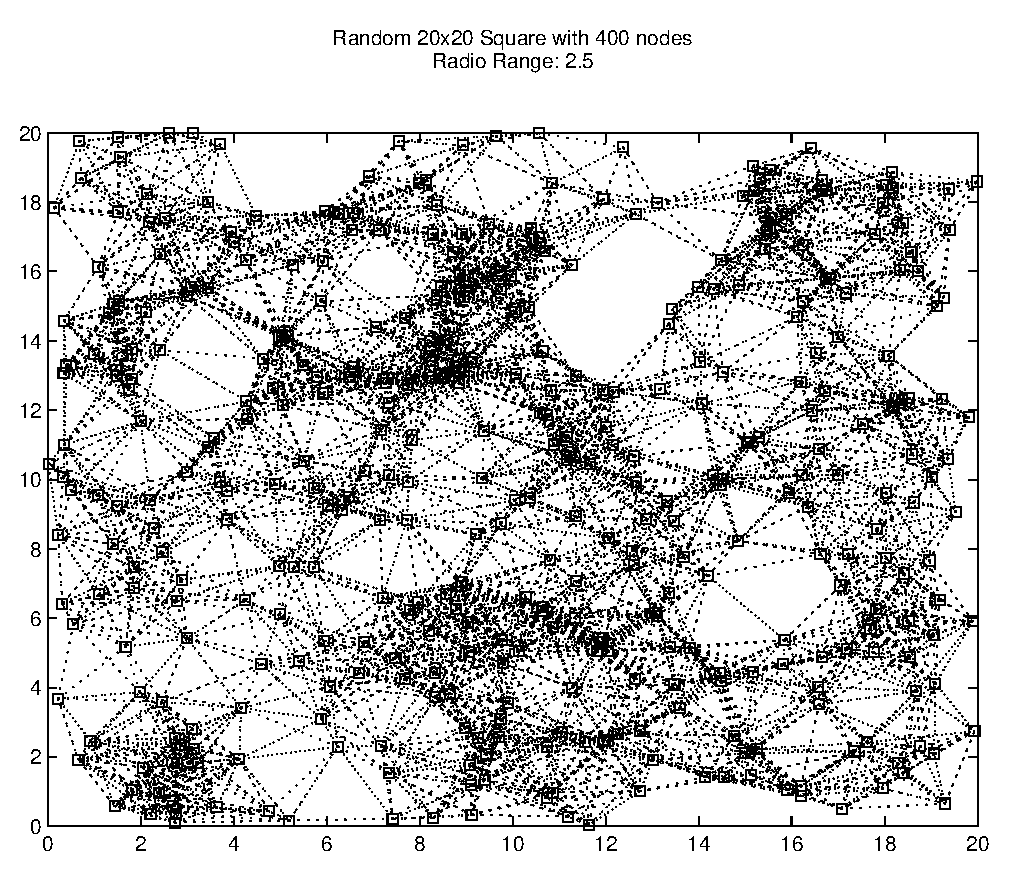
\includegraphics[width=0.75\textwidth]{network1.eps}
	\caption{The sample network used in this chapter, showing connectivity between nodes}
	\label{fig:HypothesesNetwork}
\end{figure}

Almost as important as knowing which factors effect localization is knowing which factors to ignore. The following is a summary of hypotheses of anchor node placement factors that show no or little significant correlation to location error.  The data in the following graphs is taken from a random selection of 1000 anchor sets of three nodes each for the network shown in Figure~\ref{fig:HypothesesNetwork}.  The node placement is random within the 20 by 20 square unit area, and all nodes have a radio range of 2.5 units, providing a completely connected network.

\subsection{Anchor Node Error}
The first hypothesis is to choose nodes as anchors that we expect to have high location accuracy. Because we are trying to provide an a priori design technique for network planners, the information chosen to reach the goal must be something the network planner can determine before any localization has been performed.  For this purpose we choose the number of one-hop neighbors.  Since the range-free algorithms depend heavily on network connectivity, the theory is that nodes with more neighbors will have lower location errors.  The lower error in the anchors themselves should then translate into a more accurate transformation of the entire network.

\begin{figure}
  \centering
	\subfloat[Number of Anchor Neighbors vs Location Error]{\label{fig:Neighbors}
		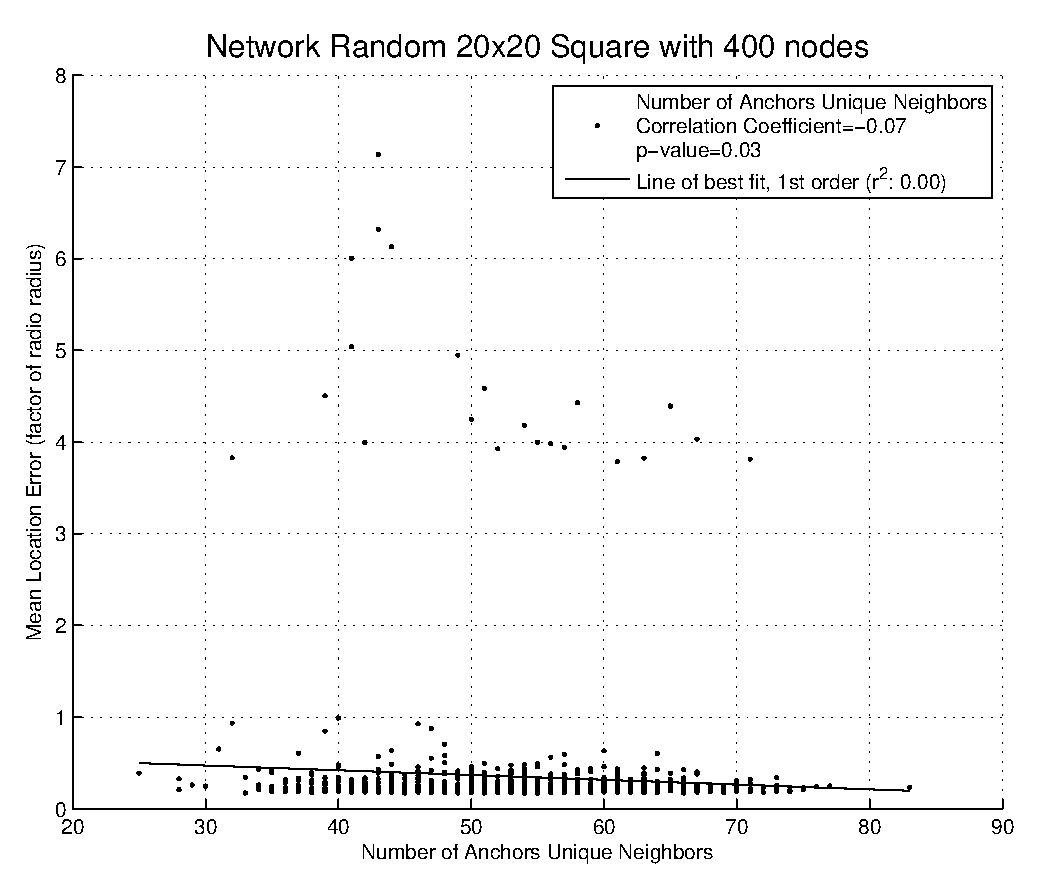
\includegraphics[width=0.5\textwidth]{numneighbors/AnchorNeighborsVsError.eps}}
	\subfloat[Number of Anchor Neighbors vs Location Error Excluding Outliers]{\label{fig:NeighborsExcluding}
		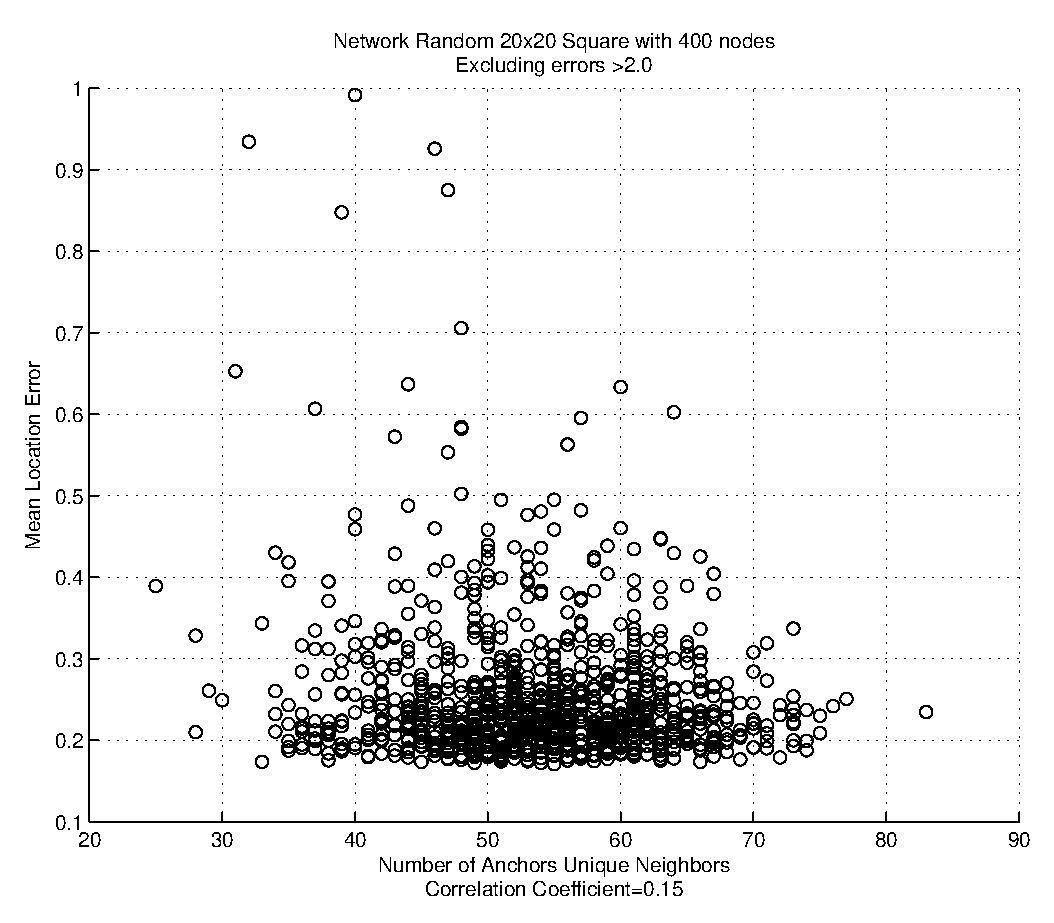
\includegraphics[width=0.5\textwidth]{numneighbors/AnchorNeighborsVsErrorExcluding.eps}}
	\\
	\subfloat[Mean Anchor Error vs Location Error]{\label{fig:AnchorError}
		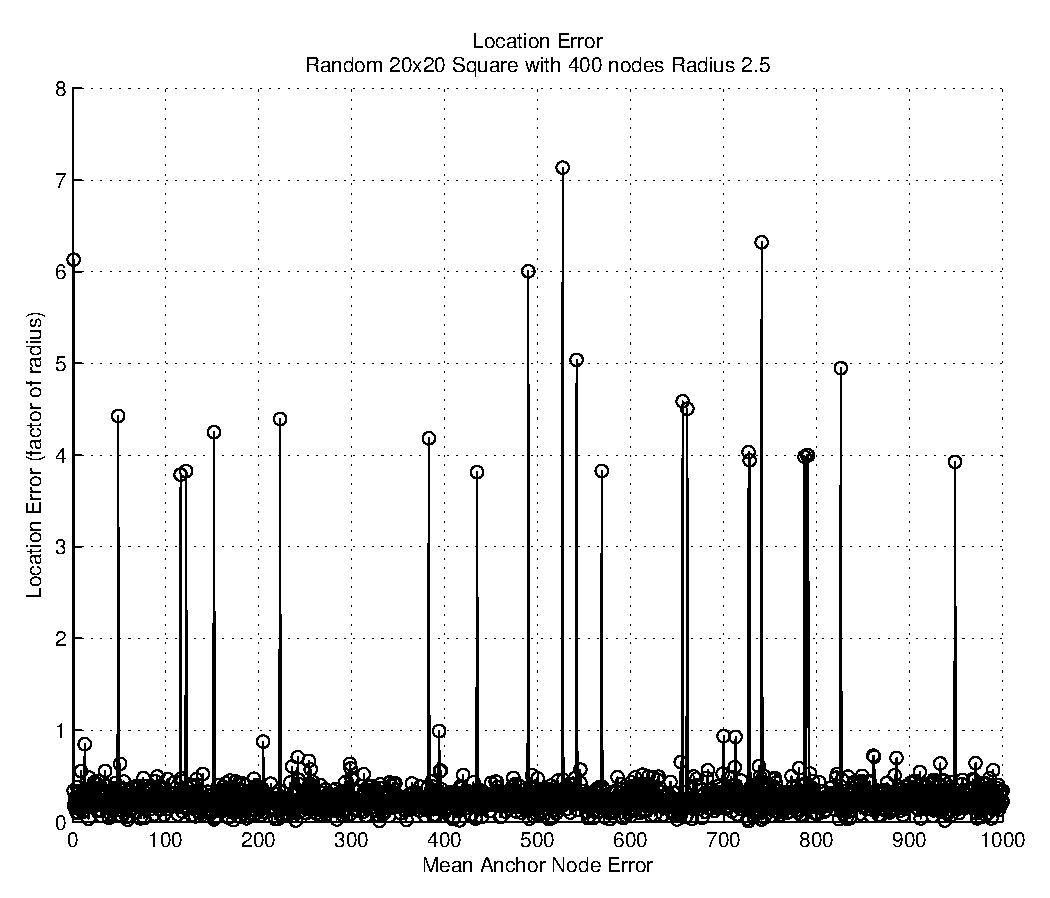
\includegraphics[width=0.5\textwidth]{numneighbors/AnchorSetErrorVsError.eps}}
	\subfloat[Mean Anchor Error vs Location Error Excluding Outliers]{\label{fig:AnchorErrorExcluding}
		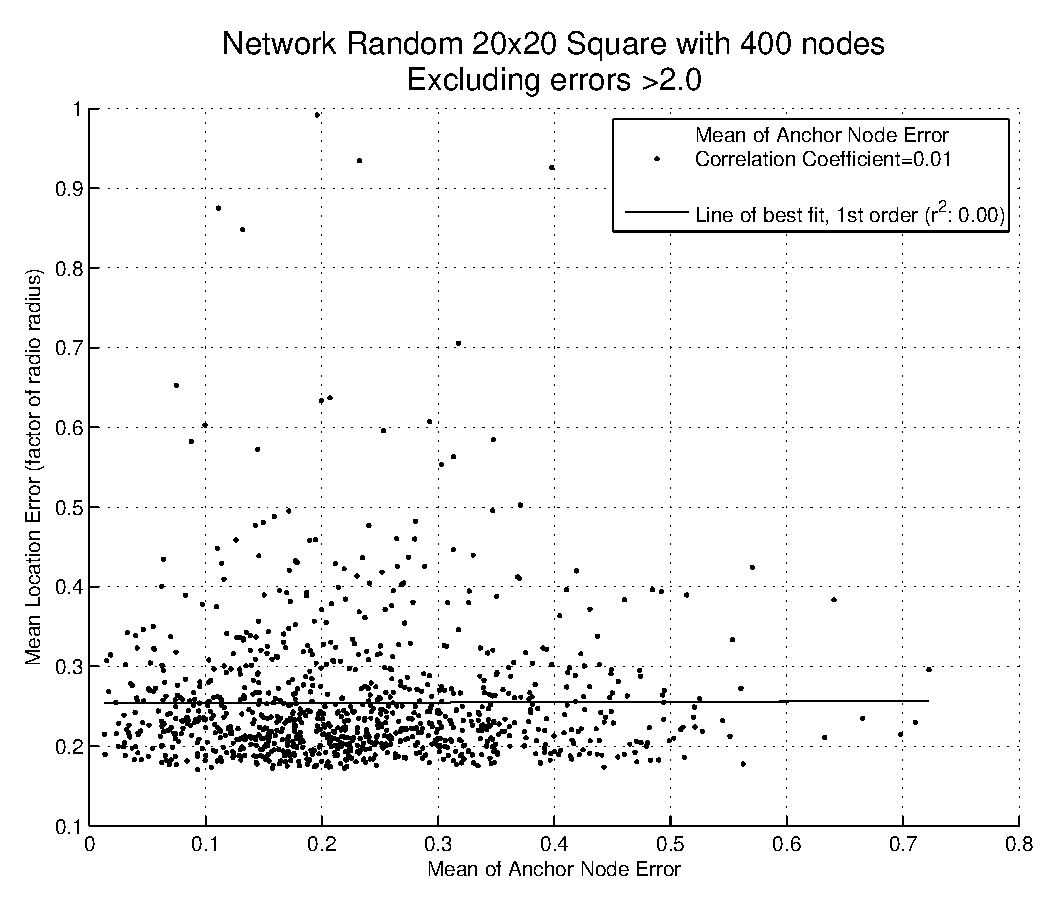
\includegraphics[width=0.5\textwidth]{numneighbors/AnchorSetErrorVsErrorExcluding.eps}}		
	\caption{}	
	\label{}
\end{figure}

Figure~\ref{fig:Neighbors} plots the sum of unique one-hop neighbors for all anchor nodes versus mean localization error.  The irregularity of the curve disproves the hypothesis. Further, the correlation coefficient, with 95\% confidence intervals, is extremely low, less than 0.1. The corresponding low \emph{p-value} of 0.03 tells us that the confidence in the lack of correlation is extremely high. Specifically, the \emph{p-value} is the probability of getting a correlation as large as the measured value 0.07 by random chance, when the true correlation is zero.  Having more neighbors means that the error of the anchor node itself has a better calculated location accuracy, but this does not translate into better network-wide accuracy.

Further, Figure~\ref{fig:AnchorError} shows the mean error of the three anchor nodes versus the mean error for all nodes in the network. Again, we have an erratic plot which disproves even the foundation of this hypothesis, namely that the location of the anchor node itself has absolutely no bearing on the overall network error. And again, the correlation coefficient is low at less than 0.15, proving again the lack of correlation, statistically.

In both plots, it is clear that a small subset of the anchor placements lead to far greater error than the norm.  Later, we will explore the cause of these outliers, but for the time being, we exclude them from the analysis as shown in Figure~\ref{fig:NeighborsExcluding} and Figure~\ref{fig:AnchorErrorExcluding}. Determining which points are outliers is quite obvious since the gap between the normal case and the small set of outliers is distinct. Therefore, rather then using a statistical calculation for the exclusion, all anchor sets with mean location error greater than two are excluded.  

Even after the outliers are excluded, no pattern emerges and the correlation coefficients remain extremely low.  Further, the line of best fit has a low r-squared value of 0.02.  Higher order best fits also show no clear correlation.

\subsection{Network Area Coverage}

Another seemingly obvious optimal anchor placement is to have the anchors as far apart as possible.  The rationale behind this hypothesis is that if a wider area of the network is covered by the anchor nodes, then the resulting calculated transformation will take into account more network variations.  

\begin{figure}
  \centering
	\subfloat[Sum of Distance]{\label{fig:AnchorDistancesSum}
		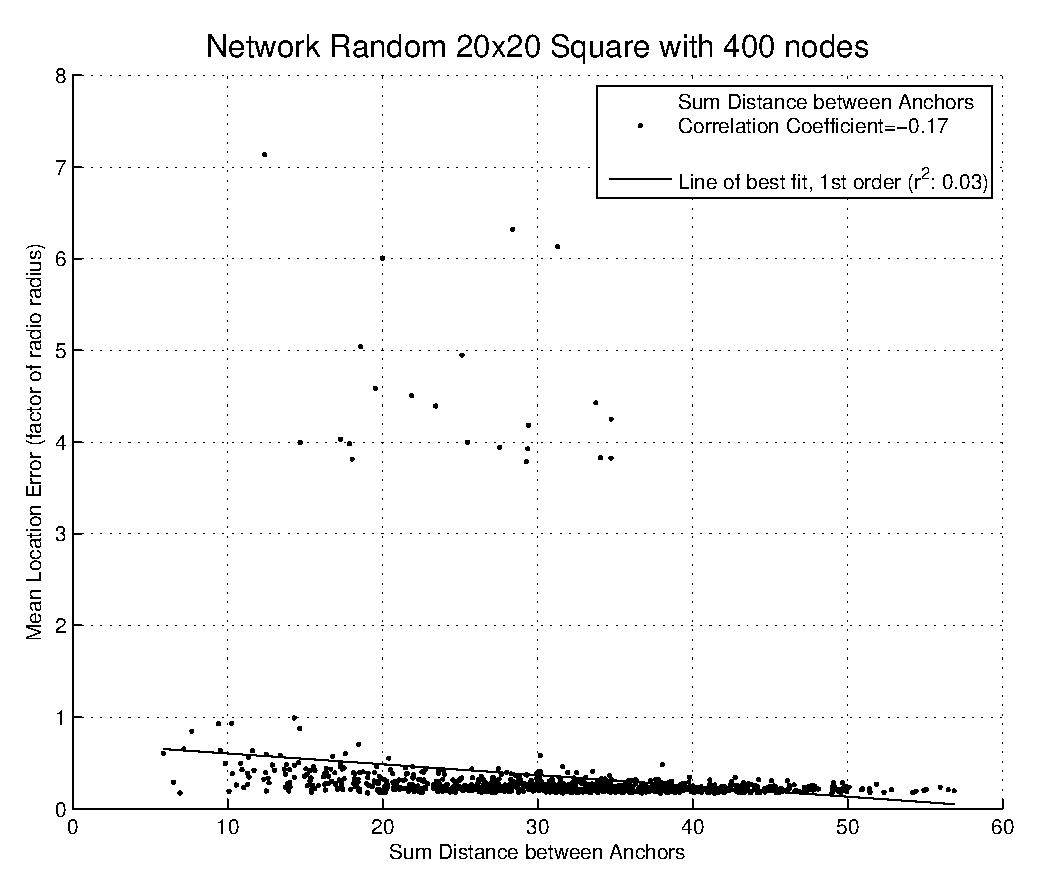
\includegraphics[width=0.5\textwidth]{distances/SumAnchorDistanceVsError.eps}}
	\subfloat[Sum of Distance, Excluding Outliers]{\label{fig:AnchorDistancesSumExcluding}
		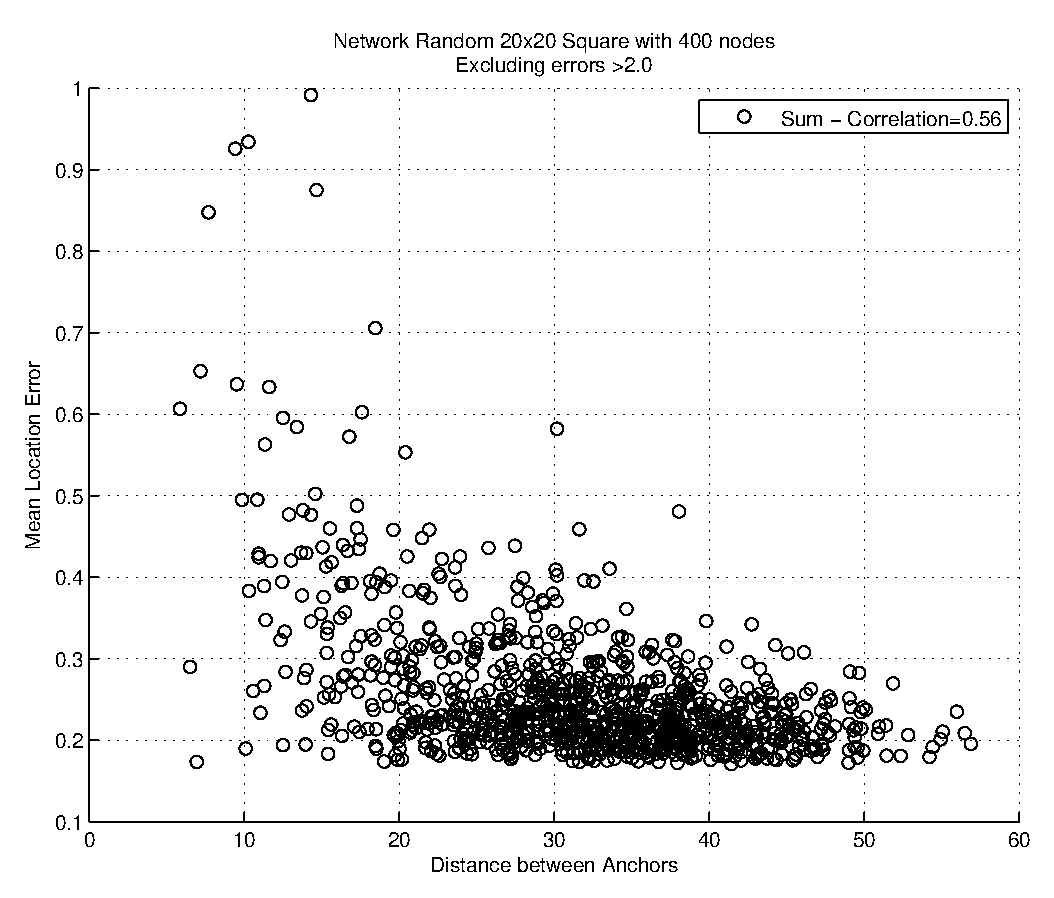
\includegraphics[width=0.5\textwidth]{distances/SumAnchorDistanceVsErrorExcluding.eps}}
		\\
	\subfloat[Minimum Distance]{\label{fig:AnchorDistancesMinimum}
		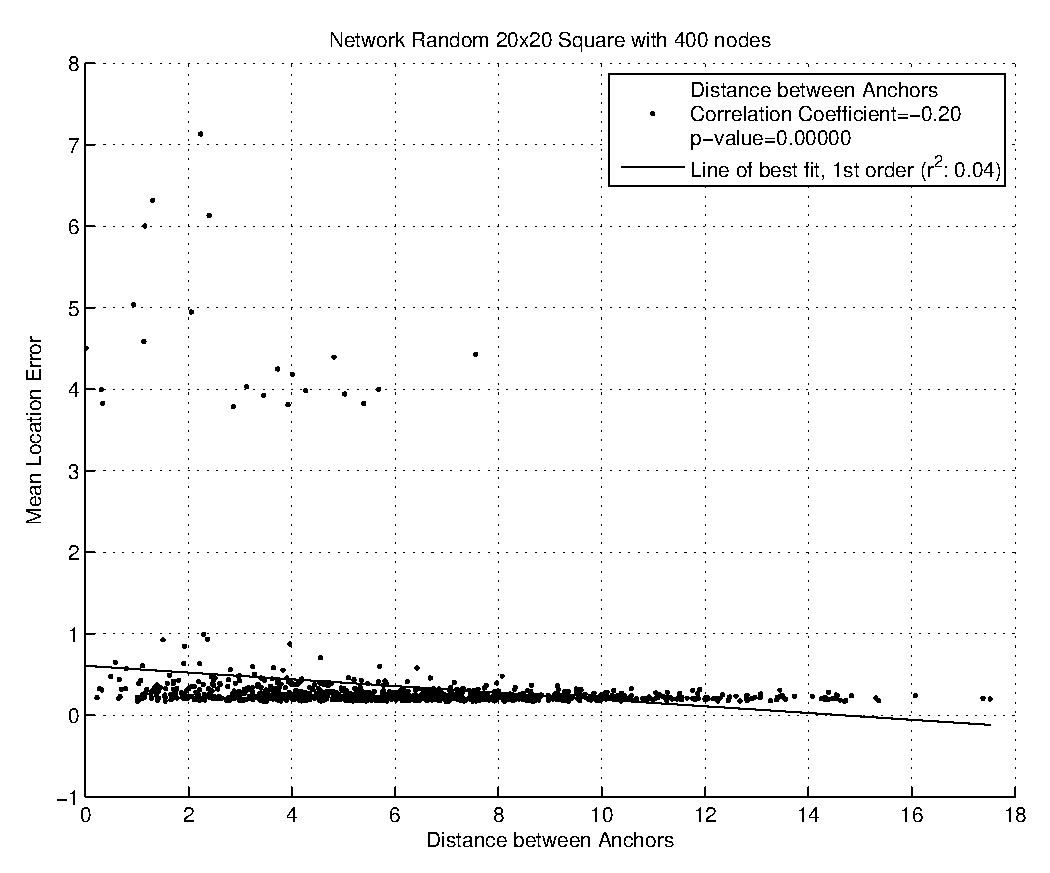
\includegraphics[width=0.5\textwidth]{distances/MinimumAnchorDistanceVsError.eps}}
	\subfloat[Minimum Distance, Excluding Outliers]{\label{fig:AnchorDistancesMinimumExcluding}
		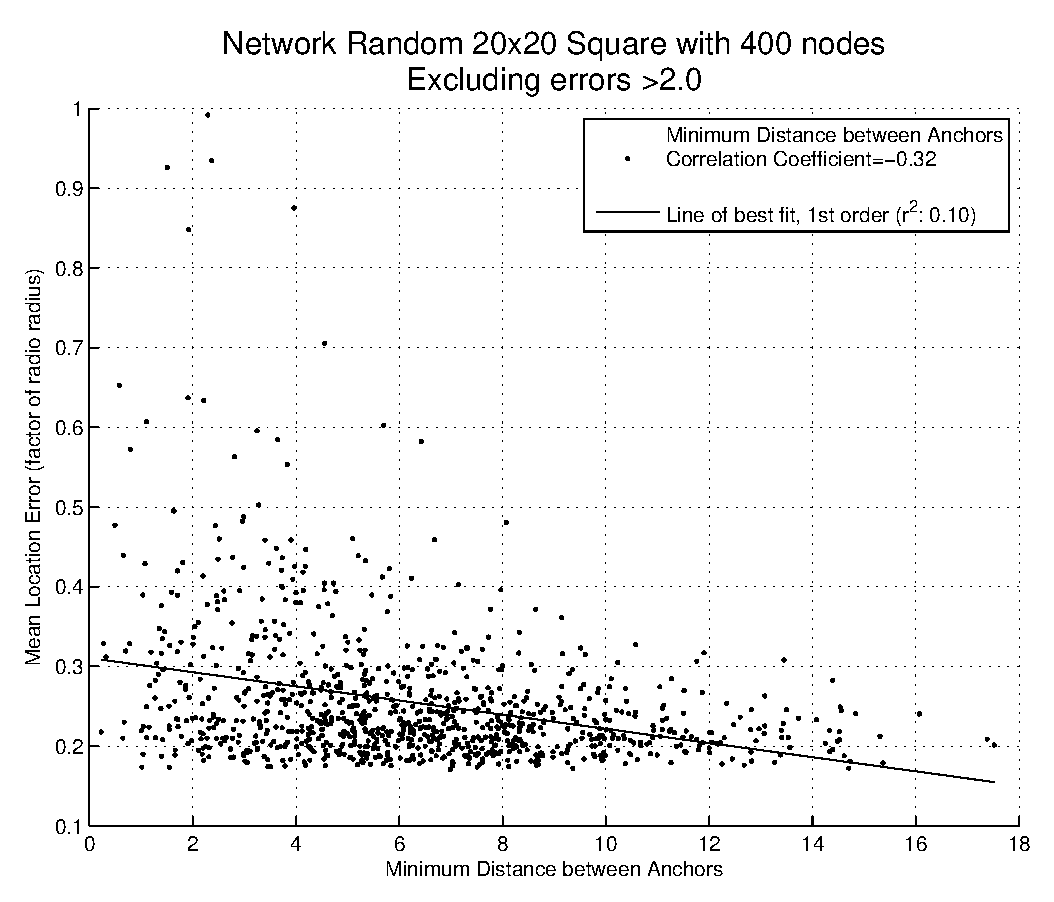
\includegraphics[width=0.5\textwidth]{distances/MinimumAnchorDistanceVsErrorExcluding.eps}}
	\caption{Distance Between Anchors}
    \label{fig:AnchorDistances}
\end{figure}

Figure~\ref{fig:AnchorDistancesSum} shows the sum of distances between each anchors versus mean localization error for that anchor set. I describe this as the sum of distances of the anchors instead of the perimeter of the triangle formed because this hypothesis investigates if the further apart the anchors are from each makes a difference. Further, the sum of distances scales for the case of more than three anchor nodes, whereas the meaning of perimeter will change the desired description. Regardless, the plot shows that again there is low correlation between the distance between anchors and the location calculation.  Further, the outliers are spread relatively evenly regardless of distance between anchor nodes.

When the outliers are excluded, as shown in Figure~\ref{fig:AnchorDistancesSumExcluding}, a moderate level of correlation is seen, with a much clear line of best fit.  The only moderate, 0.48, correlation coefficient can be explained by the lower bound for location error.  Clearly, at any distance between anchors, the lower bound can be reached as there is a virtually straight line across the bottom of the data.  However, as the distance increases between the anchor nodes, the probability of getting a high location error decreases.  

Even if the sum of distances of the anchors is high, it is possible for two anchors to be very close together and far from the third.  Therefore, the minimum distance between a pair of anchors is shown in Figure~\ref{fig:AnchorDistancesMinimum}.  Again, the correlation coefficient is low at 0.20.  However, it does appear that the outliers are slightly more likely to appear when the minimum distance between a pair of anchors is low.  Further, when outliers are excluded, as shown in Figure~\ref{fig:AnchorDistancesMinimumExcluding}, the coefficient increases to 0.32 demonstrating that perhaps the trend in thinking through these hypotheses is correct.

\subsection{Anchor Node Triangle}

Continuing the trend of trying to show some increased correlation between the anchor coverage and location error, Figure~\ref{fig:AnchorArea} plots the area of the triangle formed by the three anchor nodes versus mean location error. Figure~\ref{fig:AnchorHeight} does the same for the shortest triangle height, or in other words, a measure of the collinearity of the three anchor nodes.

While the correlation coefficients remain low, it is clear that the flatter the triangle, or the more collinear the anchor nodes, the higher chance of seeing outliers in the data with an extremely high location error. Further, after removing outliers, the slope of the best fit line is has a moderate r-squared value, giving an indication that network planners should make the anchor node triangle as spread apart as possible, or more generally, make sure the points are not collinear.

\begin{figure}
  \centering
	\subfloat[All points]{\label{fig:AnchorAreaAll}
		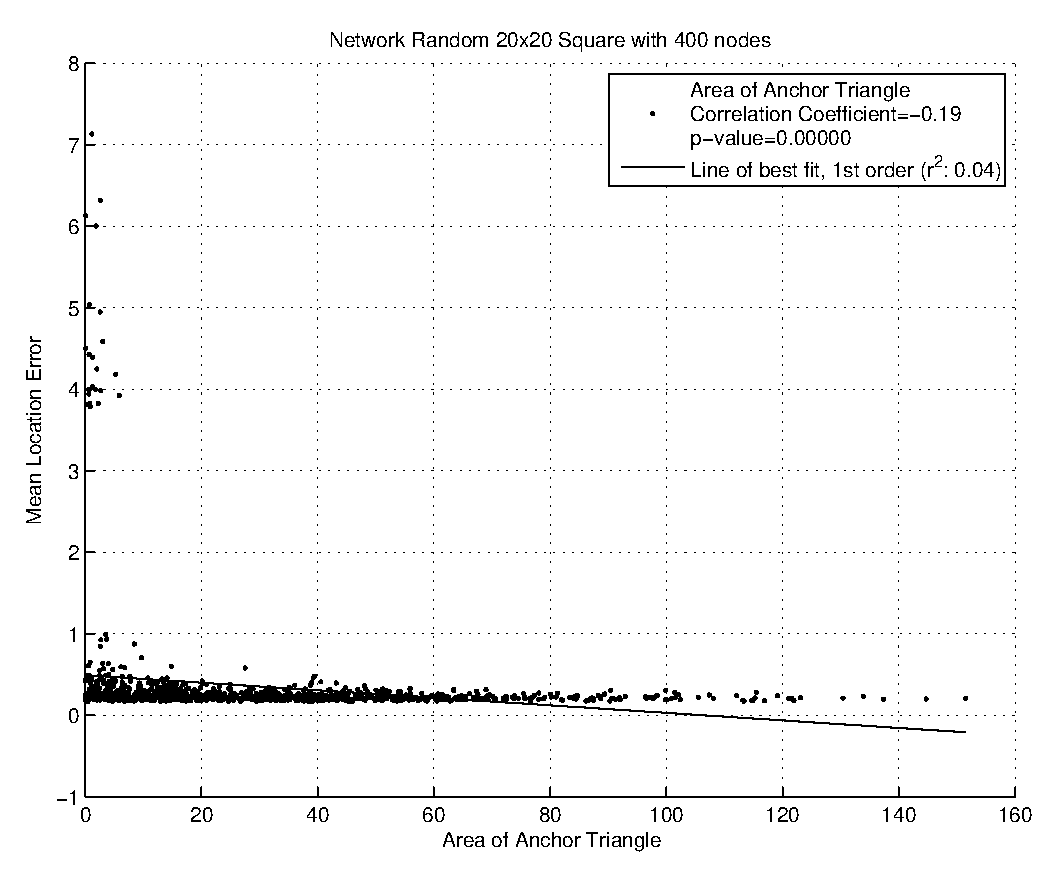
\includegraphics[width=0.5\textwidth]{areas/AnchorAreaVsError.eps}}
	\subfloat[Excluding outliers]{\label{fig:AnchorAreaExcluding}
		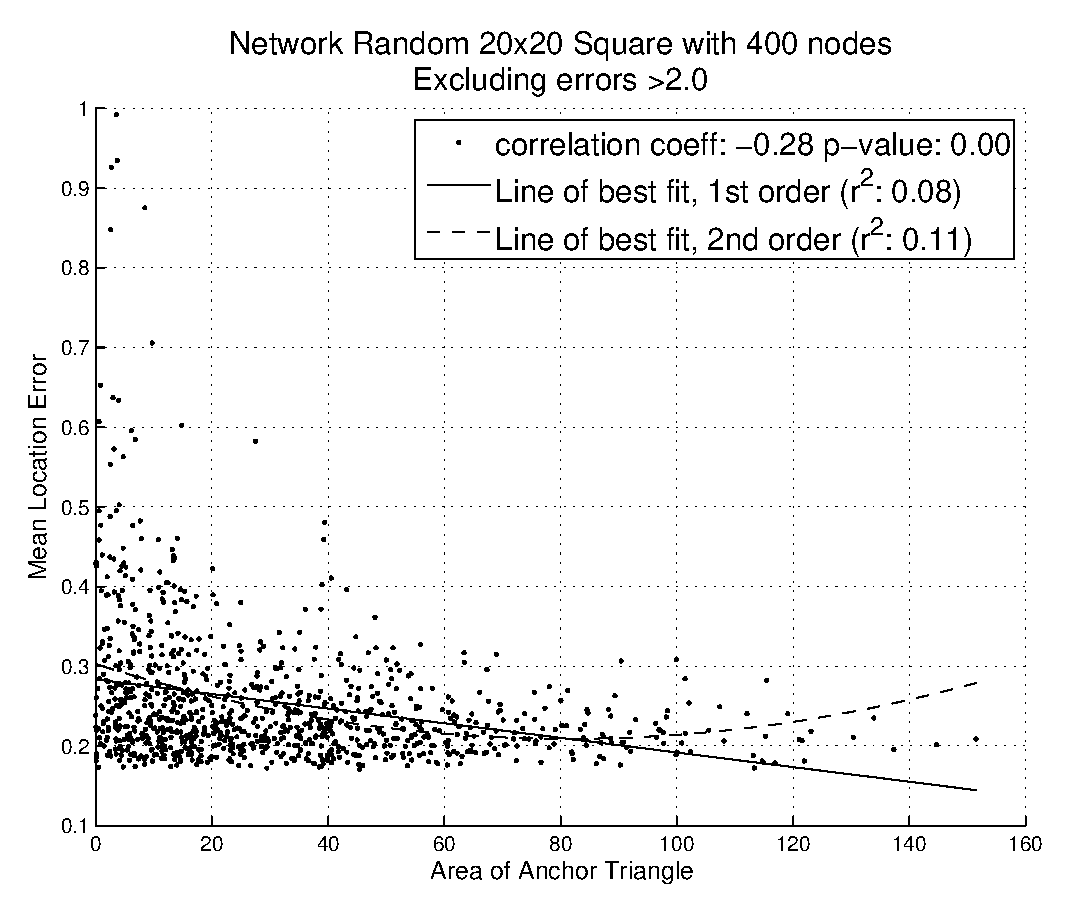
\includegraphics[width=0.5\textwidth]{areas/AnchorAreaVsErrorExcluding.eps}}
	\caption{Area of Anchor Triangle vs Location Error}	    
	\label{fig:AnchorArea}
\end{figure}

\begin{figure}
  \centering
	\subfloat[All points]{\label{fig:AnchorHeightAll}
		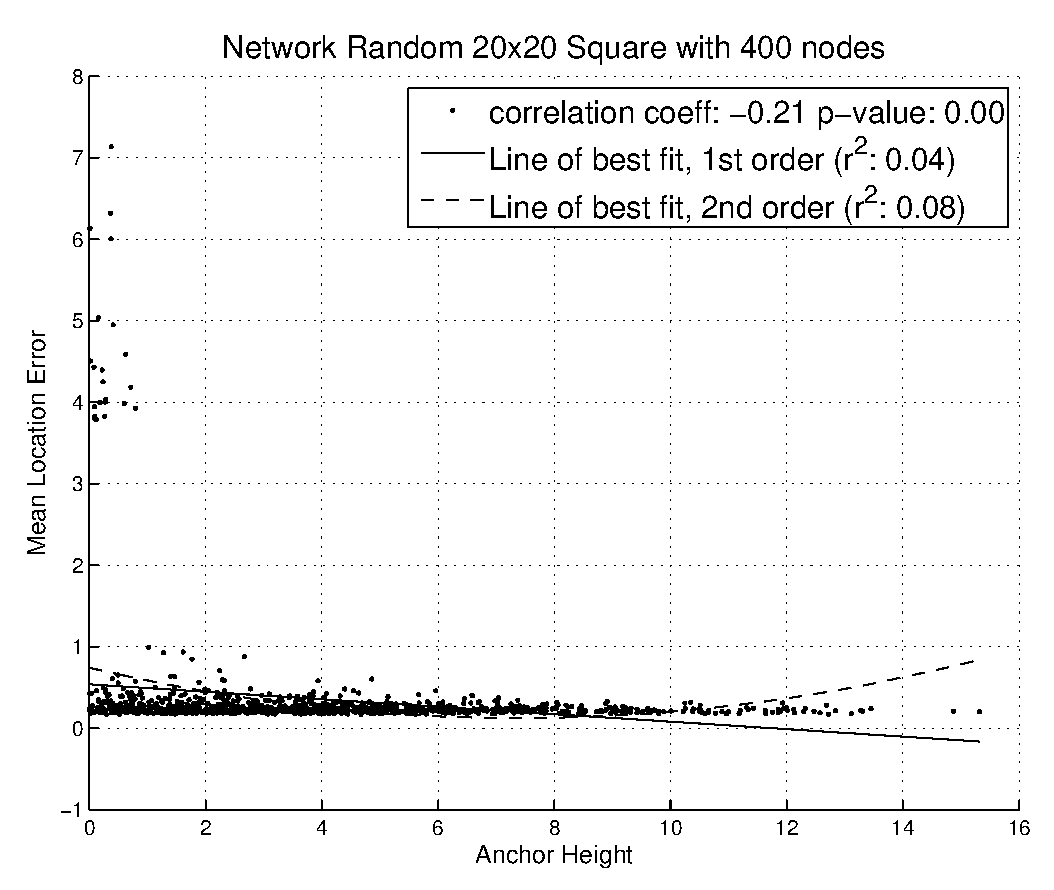
\includegraphics[width=0.5\textwidth]{heights/AnchorHeightVsError.eps}}
	\subfloat[Excluding outliers]{\label{fig:AnchorAreaExcluding}
		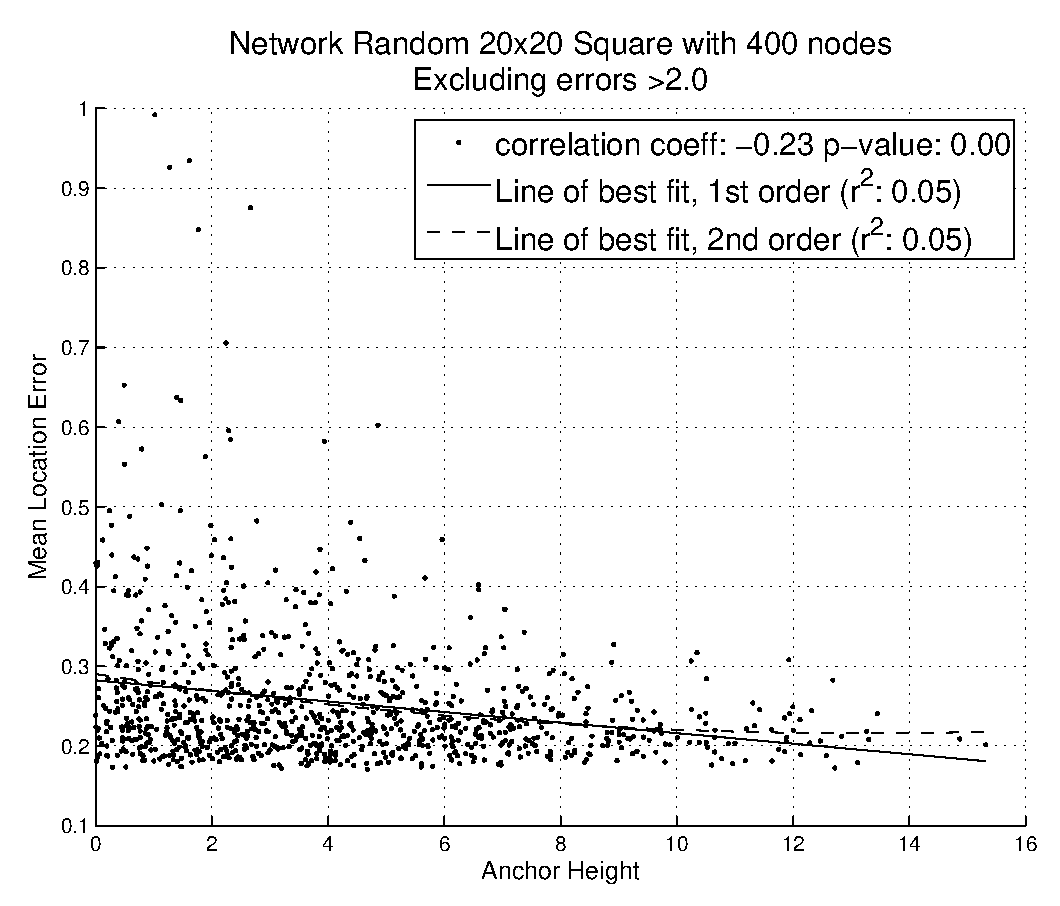
\includegraphics[width=0.5\textwidth]{heights/AnchorHeightVsErrorExcluding.eps}}
	\caption{Minimum Height of Anchor Triangle vs Location Error}	    
	\label{fig:AnchorHeight}
\end{figure}
